\documentclass{standalone}

\begin{document}

\section{Feature Analysis and Engineering}

The data comes in the traditional Kaggle form of one training and test file
each: \lstinline{train.csv} and \lstinline{test.csv}. Each row corresponds to a
specific policy holder and the columns describe their features. The target
variable is named \lstinline{target} here and it indicates whether this policy
holder made an insurance claim in the past.

\subsection{Data Overview}

In total, there are $595212$ training data instances and $892816$ testing data instance. Since it's a competition, testing data had no \lstinline{target} label. We cannot test our model accuracy based on testing data. In stead, we would use k-fold and cross validation on the training data to evaluate our model, which is discussed in more detail in \cref{evam}.

In the train and test data, features that belong to similar groupings are
tagged as such in the feature names (e.g., \lstinline{ind}, \lstinline{reg},
\lstinline{car}, \lstinline{calc}). In addition, feature names include the
postfix \lstinline{bin} to indicate binary features and \lstinline{cat} to
indicate categorical features. Features without these designations are either
continuous or ordinal. Feature count in each category and type are shown in \cref{feature_count}.

\begin{table}[!h]
\renewcommand{\arraystretch}{1.3}
\caption{Feature Counts in Each Category and Type}\label{feature_count}
\centering
\begin{tabular}{c|cccc}
\hline
\bfseries Type & \bfseries  Binary & \bfseries  Categorical & \bfseries  Numeric & \bfseries Total \\ \hline
\ttfamily ind & 11 & 3 & 4 & 18 \\ \hline
\ttfamily reg & 0 & 0 & 3 & 3 \\ \hline
\ttfamily car & 0 & 11 & 5 & 16 \\ \hline
\ttfamily calc & 6 & 0 & 14 & 20 \\ \hline
\end{tabular}

% \begin{tabular}{c|cccc}
% \hline
% Type & \bfseries ind & \bfseries reg & car & calc \\ \hline
% Binary & & & & \\ \hline
% Categorical & & & & \\ \hline
% Continuous & & & & \\ \hline
% Ordinal & & & & \\ \hline
% \end{tabular}
\end{table}

Although feature's categories are provided, the meaning of each feature remains unknown. Some participants have guessed the meaning of several features, for example the \emph{binary} variables  \lstinline{ps_ind_06-10} are \emph{one-hot encoded}, and \lstinline{ps_car_13} might be car's mileage.
Our experiment show that some of the assumptions are plausible, however, we did not rely on these information to build our model.

\subsection{Distribution Analysis}

Features' distribution for \lstinline{ind}, \lstinline{reg}, \lstinline{car}, \lstinline{calc} are shown as histograms in \cref{hist_ind}, \cref{hist_reg}, \cref{hist_car} and \cref{hist_calc} respectfully.

\begin{figure*}[!htb]
\centering
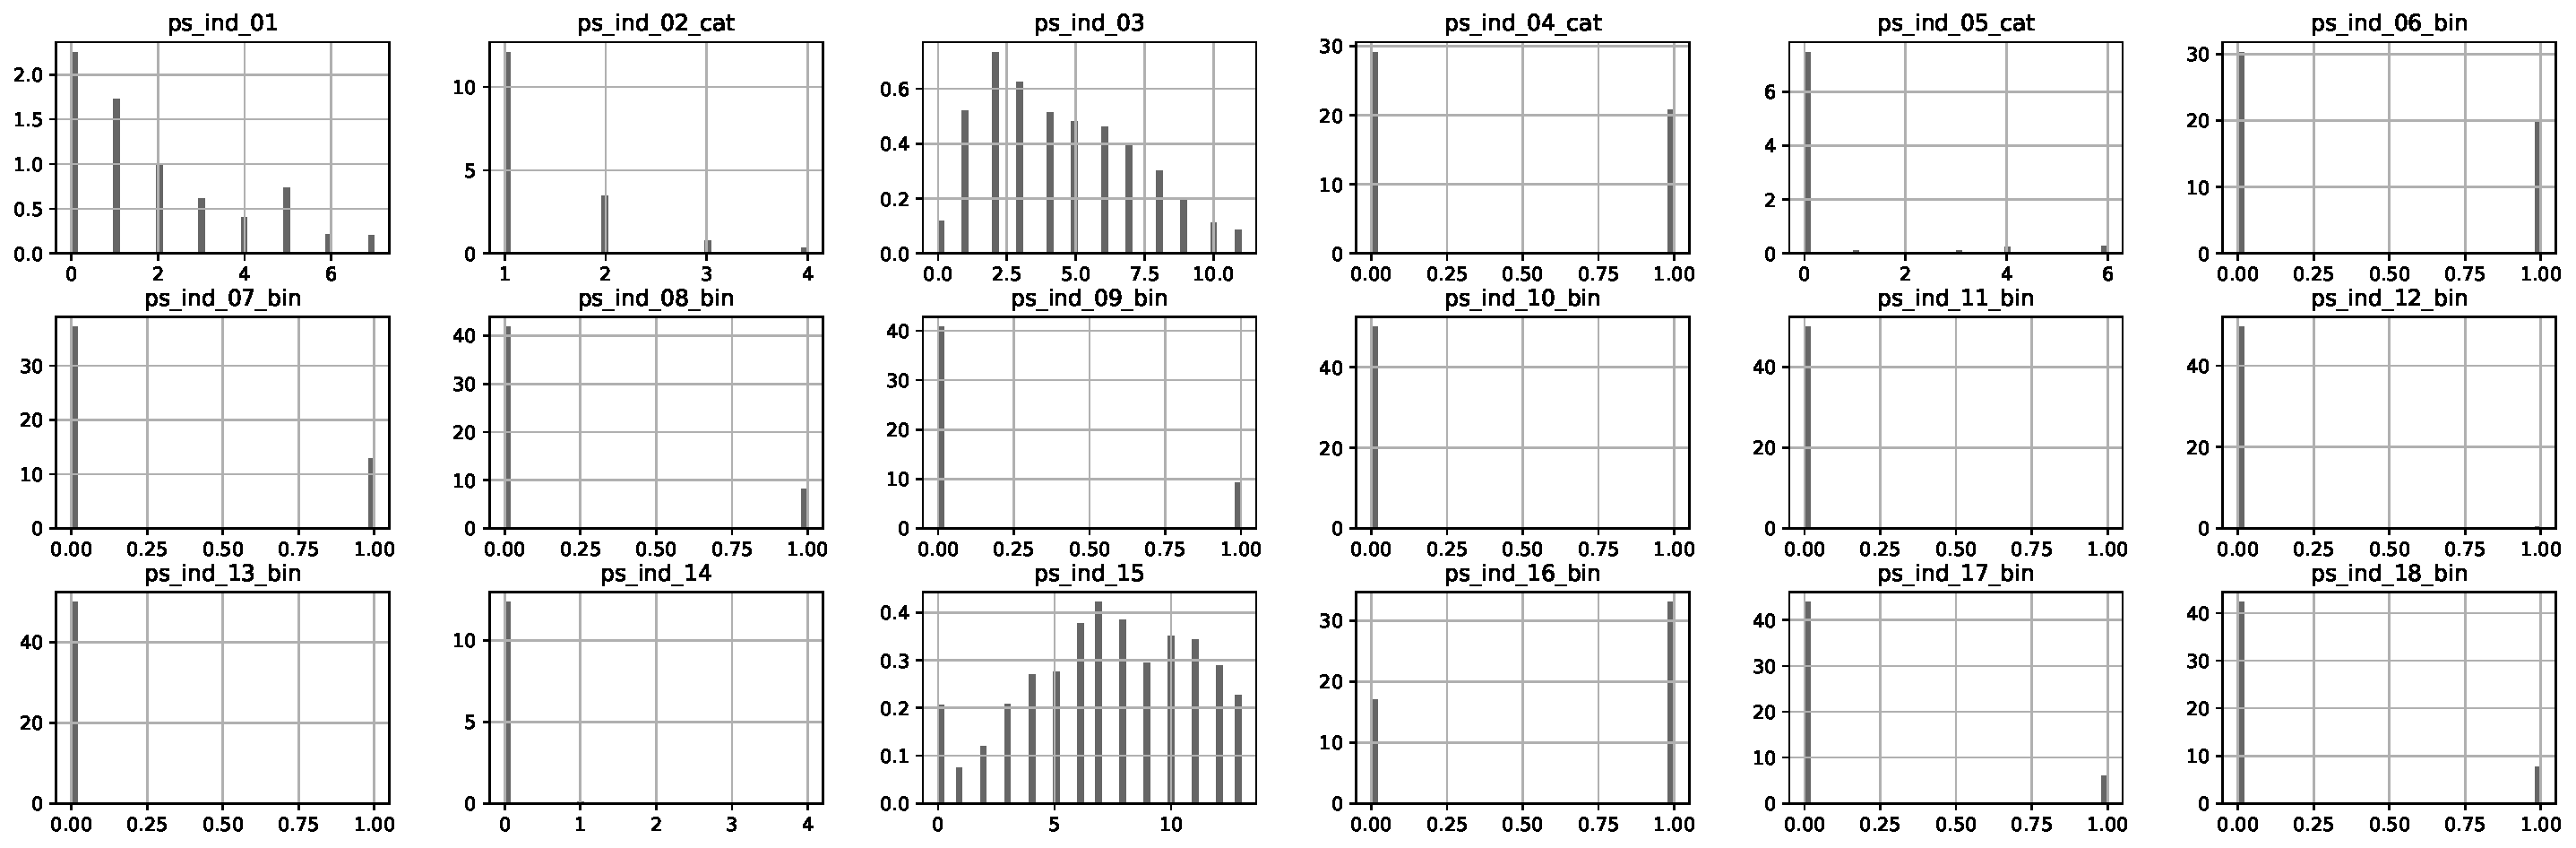
\includegraphics[width=\textwidth]{fig/ind_col.pdf}
\caption{Histogram for the \lstinline{ind} Attributes.}
\label{hist_ind}
\end{figure*}

\begin{figure}[!ht]
\centering
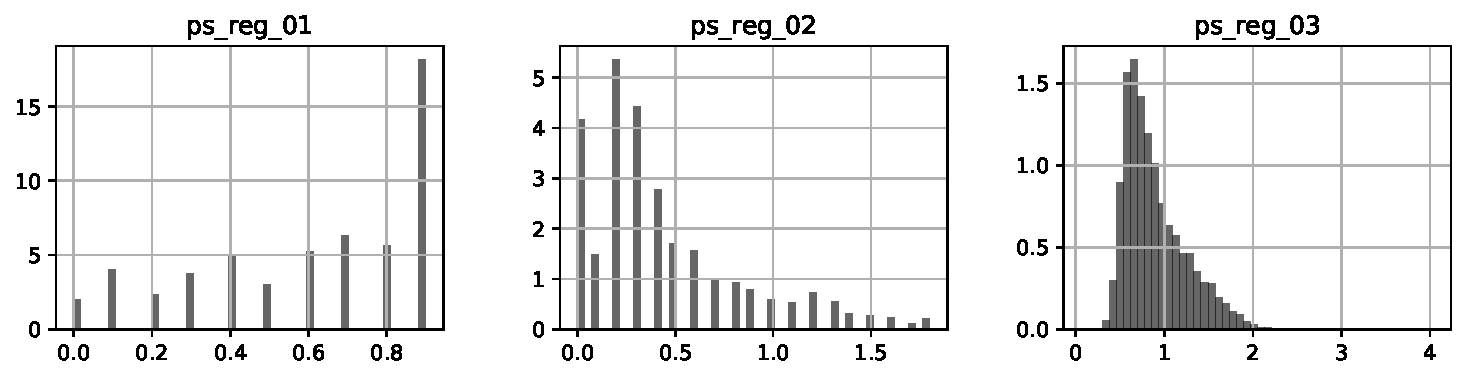
\includegraphics[width=.5\textwidth]{fig/reg_col.pdf}
\caption{Histogram for the \lstinline{reg} Attributes.}
\label{hist_reg}
\end{figure}

\begin{figure*}[!ht]
\centering
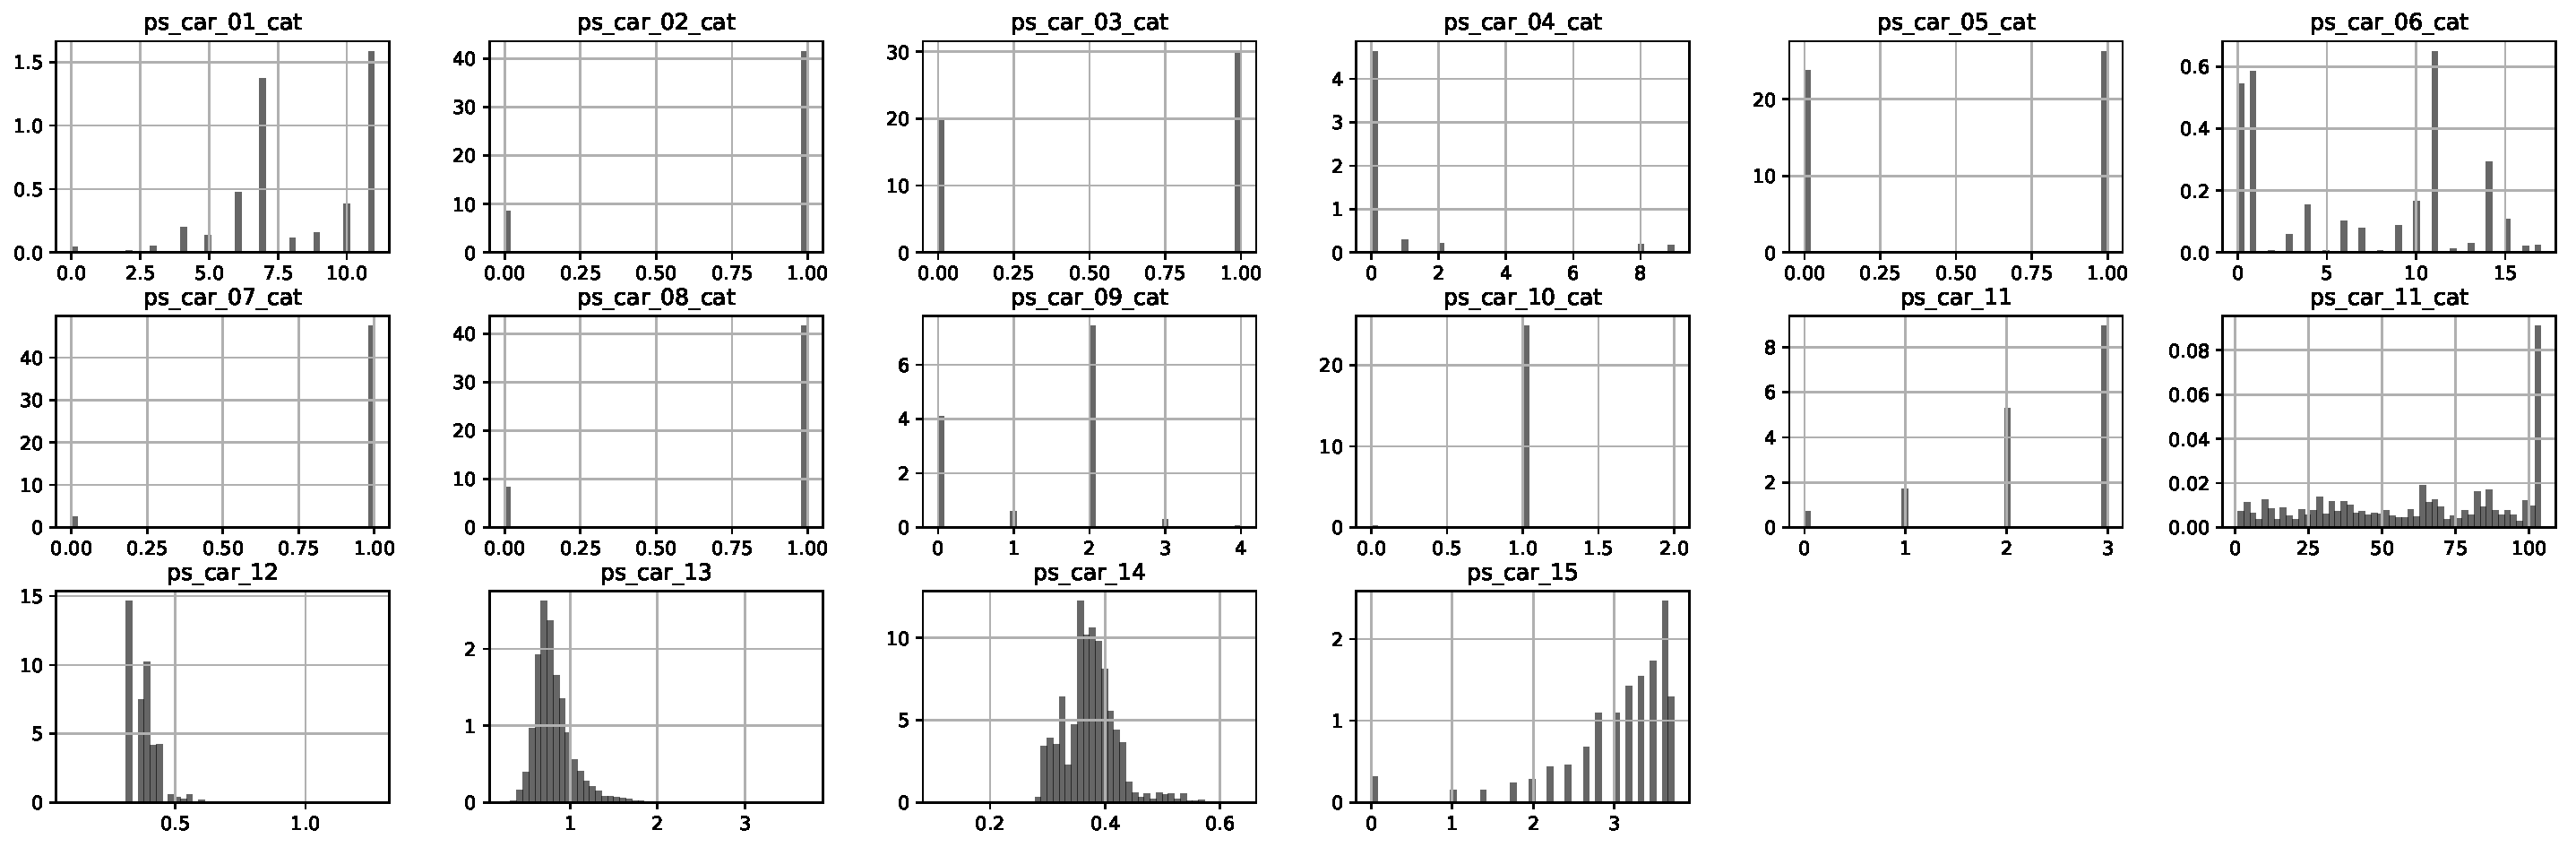
\includegraphics[width=\textwidth]{fig/car_col.pdf}
\caption{Histogram for the \lstinline{car} Attributes.}
\label{hist_car}
\end{figure*}

\begin{figure*}[!ht]
\centering
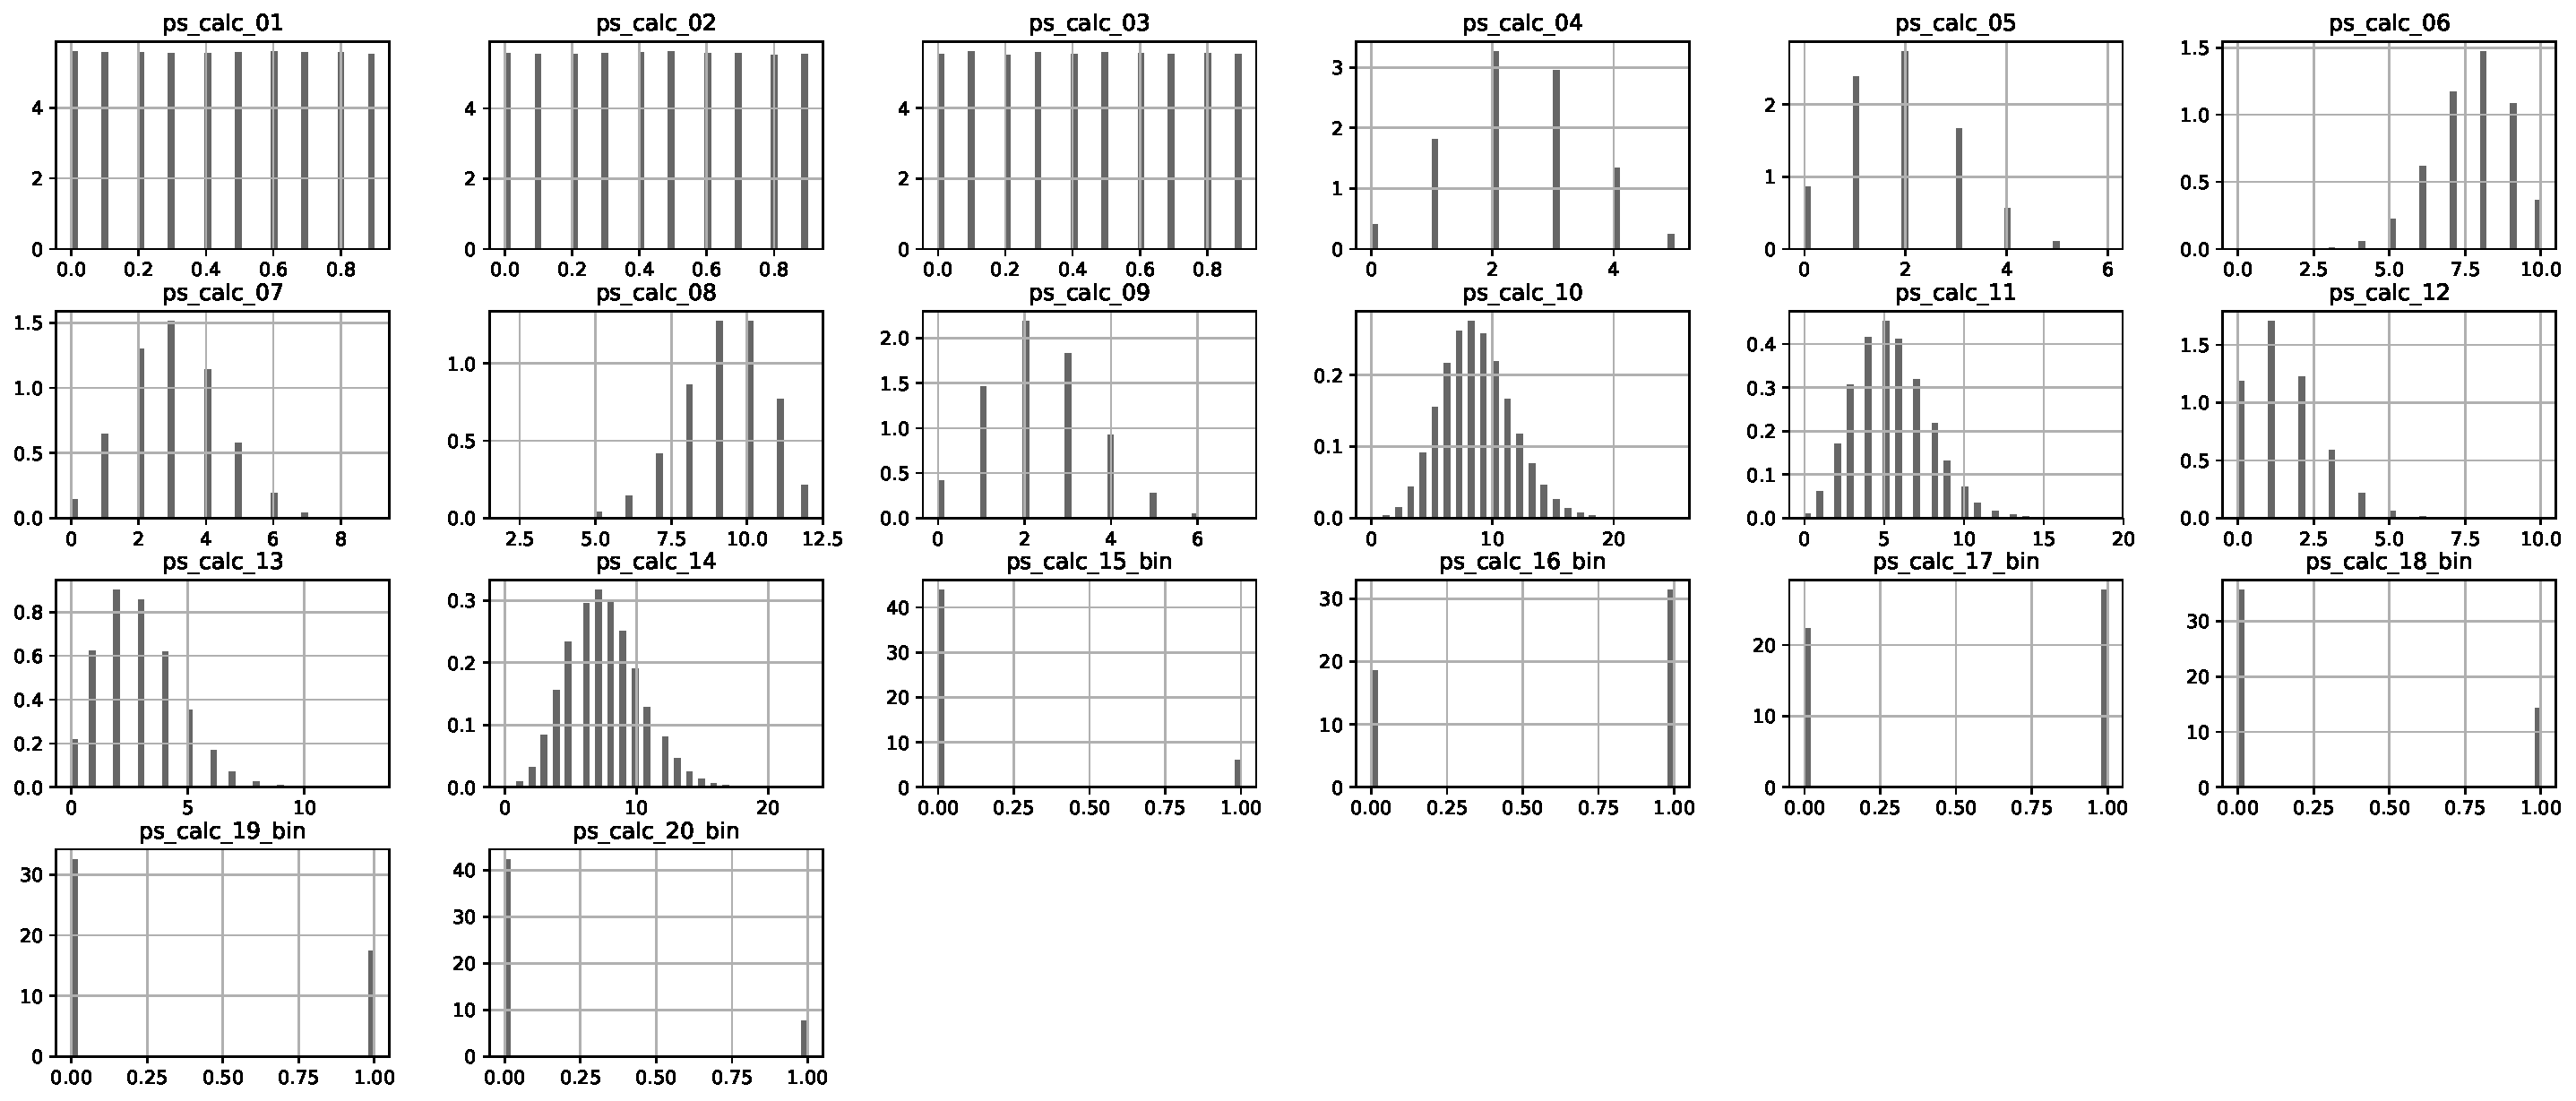
\includegraphics[width=\textwidth]{fig/calc_col.pdf}
\caption{Histogram for the \lstinline{calc} Attributes.}
\label{hist_calc}
\end{figure*}

From histograms, we may conclude the following:
\begin{itemize}
\item Some binary features are dominated by \lstinline{True} (\lstinline{False}), for example \lstinline{ps_ind_06-10}.
\item Some features' distribution are fairly even, for example \lstinline{ps_calc_01}, \lstinline{ps_calc_02} and \lstinline{ps_calc_03}.
\end{itemize}

It might seem plausible to discard these features in training phase. But the deletion requires more careful consideration. As mentioned above, \lstinline{ps_ind_06-10} might be \emph{one-hot encoded}, thus, all these four features would be naturally exclusive of each other.

\subsection{Correlation Analysis}

Features' Correlation within each category, i.e., \lstinline{ind}, \lstinline{reg}, \lstinline{car}, \lstinline{calc} are shown as histograms in \cref{corr_ind}, \cref{corr_reg}, \cref{corr_car} and \cref{corr_calc} respectfully.


\begin{figure}[!t]
\centering
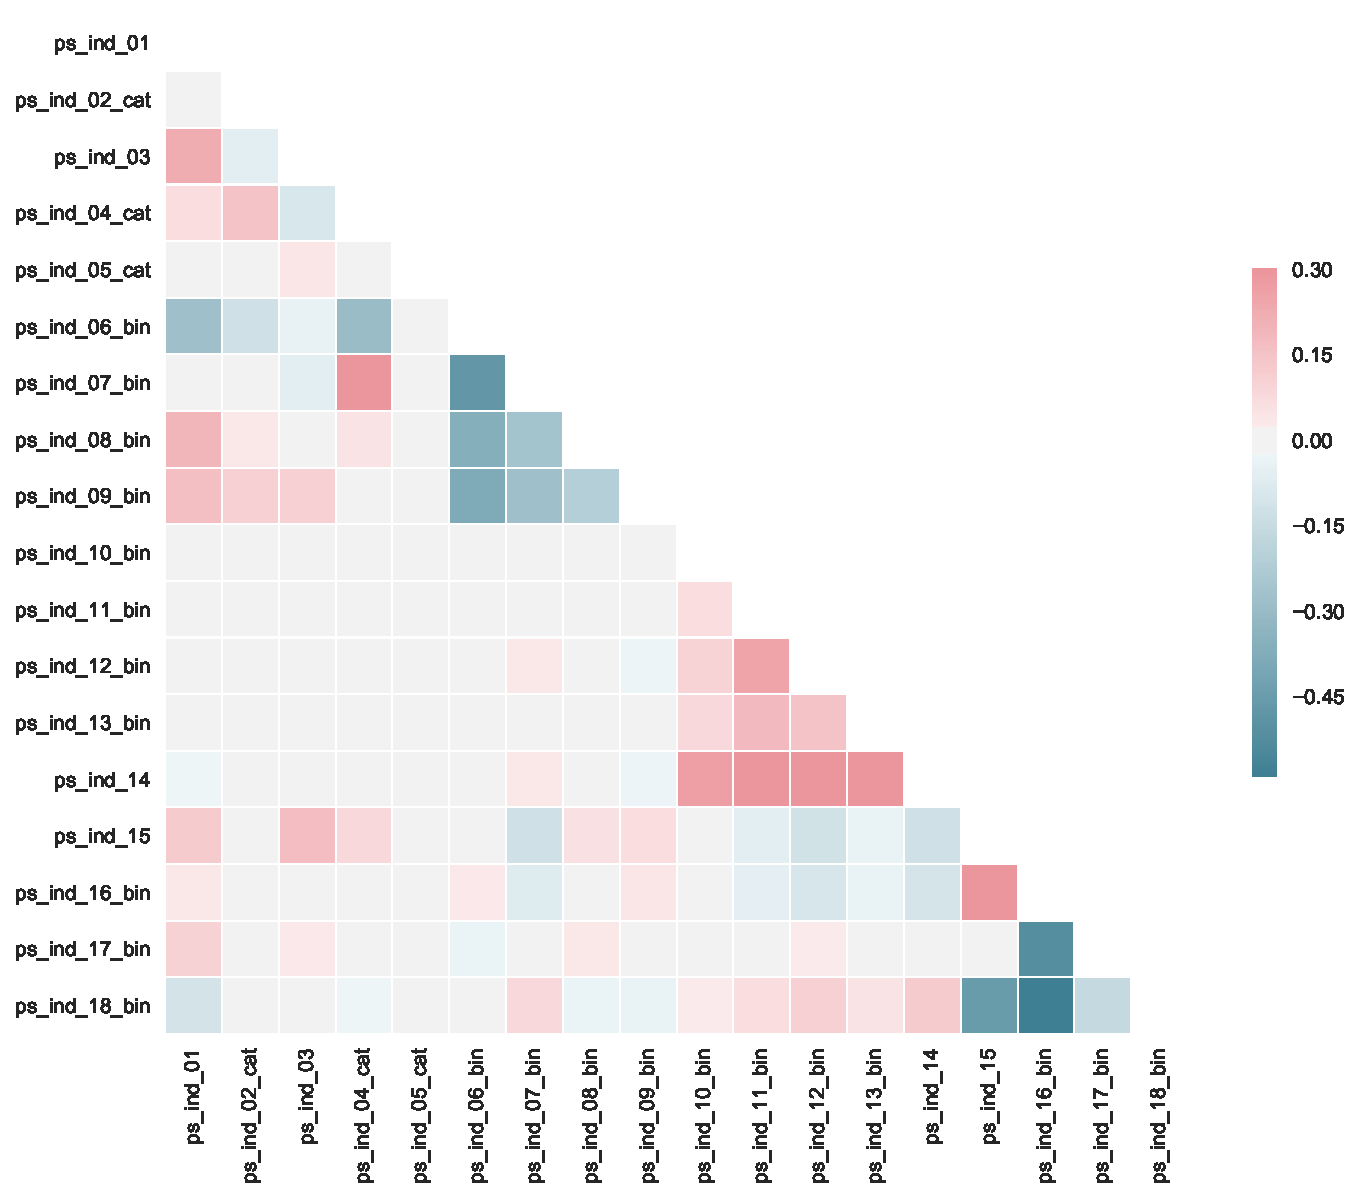
\includegraphics[width=.5\textwidth]{fig/corr_ind_col.pdf}
\caption{Correlation for the \lstinline{ind} Attributes.}
\label{corr_ind}
\end{figure}

\begin{figure}[!t]
\centering
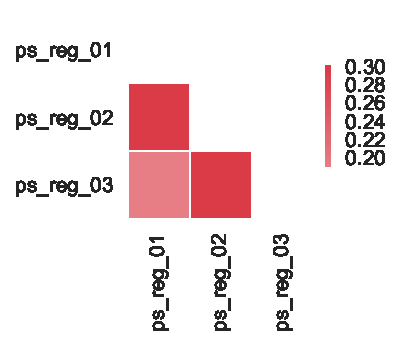
\includegraphics[width=.2\textwidth]{fig/corr_reg_col.pdf}
\caption{Histogram for the \lstinline{reg} Attributes.}
\label{corr_reg}
\end{figure}

\begin{figure}[!t]
\centering
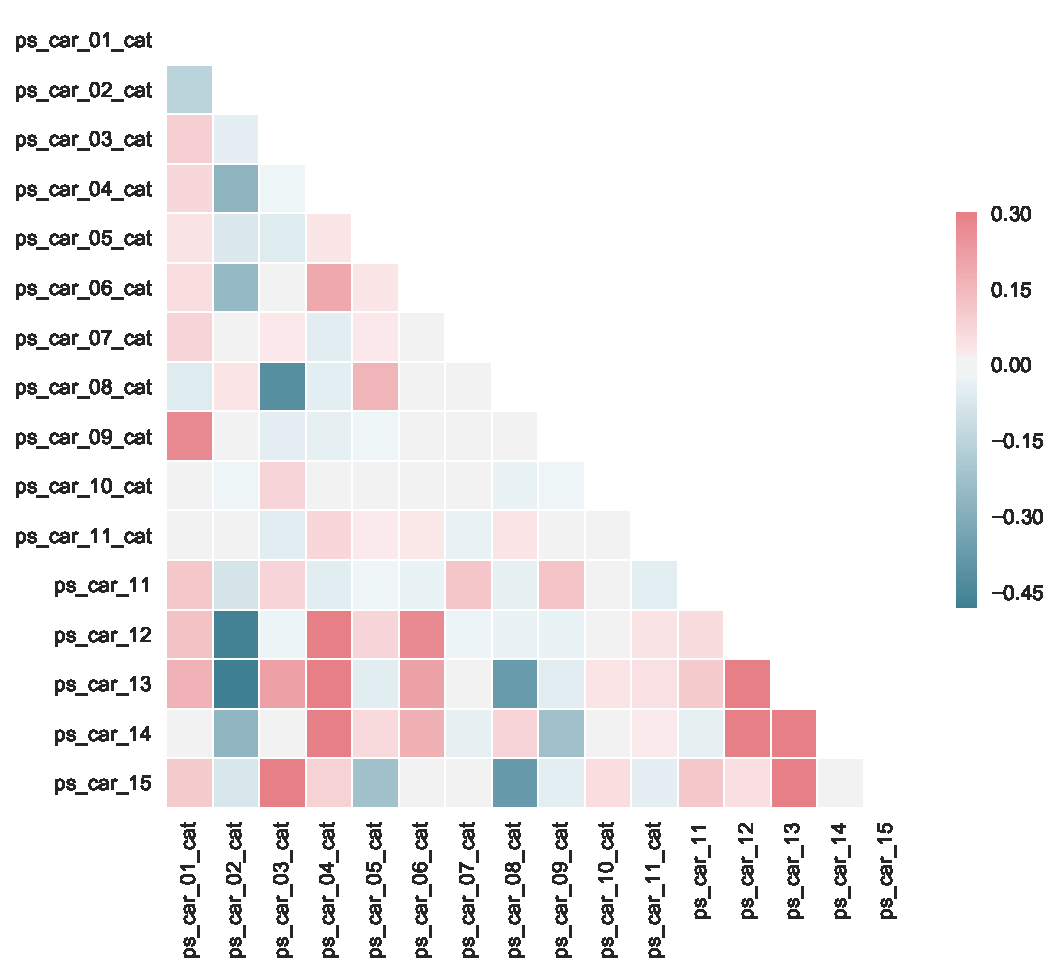
\includegraphics[width=.5\textwidth]{fig/corr_car_col.pdf}
\caption{Histogram for the \lstinline{car} Attributes.}
\label{corr_car}
\end{figure}

\begin{figure}[!t]
\centering
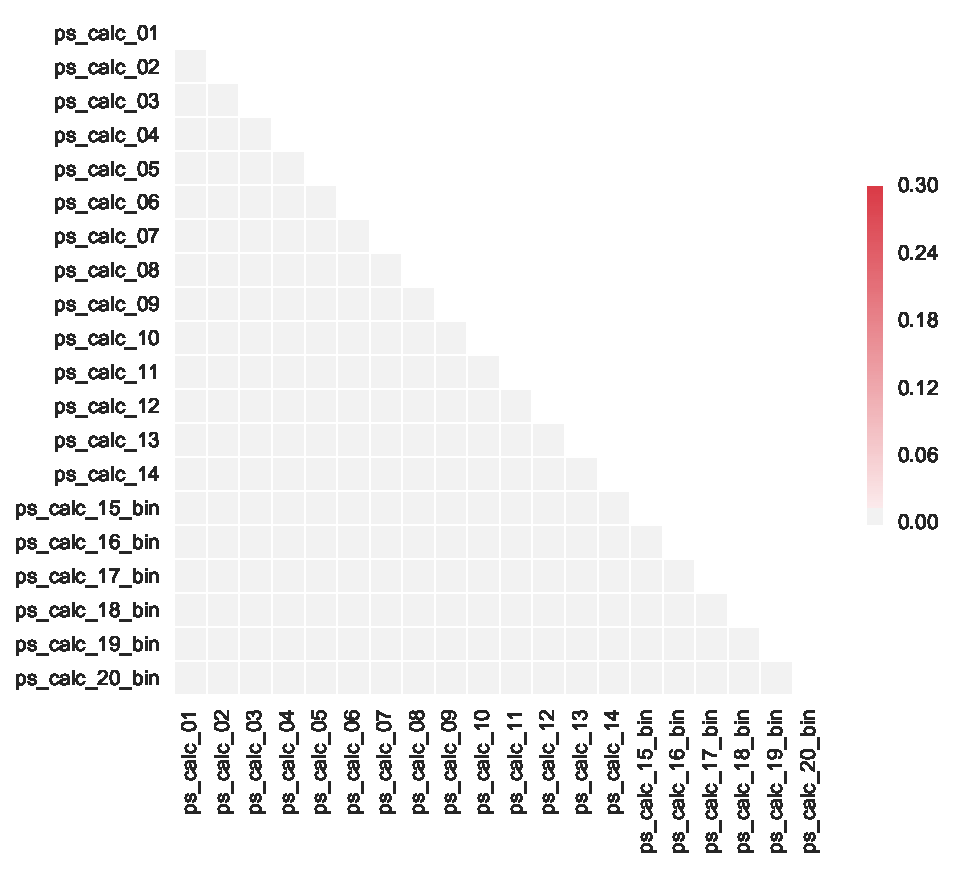
\includegraphics[width=.5\textwidth]{fig/corr_calc_col.pdf}
\caption{Histogram for the \lstinline{calc} Attributes.}
\label{corr_calc}
\end{figure}

From correlation plot, we can conclude that strong correlation did not exist.
It it not possible to conduct any dimension reduction based on correlations
between features.

\subsection{Missing Value Mechanism and Data Imputation}

Values of -1 indicate that the feature was missing from
the observation. Missing values count in each feature is shown in \cref{missing_count}:

\begin{table}[!h]
\renewcommand{\arraystretch}{1.3}
\caption{Missing Value Counts in Each Feature}\label{missing_count}
\centering
\begin{tabular}{l|r|r}
\toprule
\bfseries Feature Name & \bfseries Count & \bfseries Percentage \\
\midrule
\verb|ps_ind_02_cat|  &      216 & 0.0363\%\\
\verb|ps_ind_04_cat|  &       83 & 0.0139\%\\
\verb|ps_ind_05_cat|  &     5809 & 0.9760\%\\
\verb|ps_reg_03|      &   107772 & 18.1065\%\\
\verb|ps_car_01_cat|  &      107 & 0.0180\%\\
\verb|ps_car_02_cat|  &        5 & 0.0008\%\\
\verb|ps_car_03_cat|  &   411231 & 69.0898\%\\
\verb|ps_car_05_cat|  &   266551 & 44.7825\%\\
\verb|ps_car_07_cat|  &    11489 & 1.9302\%\\
\verb|ps_car_09_cat|  &      569 & 0.0956\%\\
\verb|ps_car_11|      &        5 & 0.0008\%\\
\verb|ps_car_12|      &        1 & 0.0002\%\\
\verb|ps_car_14|      &    42620 & 7.1605\%\\
\bottomrule
\end{tabular}
\end{table}

There are several approaches to handle missing values\cite{Intro:Missing}:

\begin{itemize}
\item Deletion methods: cases with missing values are discarded, the analyses are restricted to cases that have
complete data.
\item Single imputation methods: imputes (i.e., \emph{fills in}) the missing data with seemingly suitable replacement values. Mean, median and mode are the most popular averaging techniques to use\cite{Missing:Howto}.
\item Multiple imputation methods: creates several copies of the data set, each containing different
imputed values. These method has greater performance but is harder to implemented.
\end{itemize}

From the table we can see that, most features have no missing value (only 13 features out of 51 have).
Some features only have a small amount of instances with missing value (\lstinline{ps_car_02_cat} and \lstinline{ps_car_11} have 5 missing value and \lstinline{ps_car_12} have only 1).

Based on these observation, we handled the missing values as follow:

\begin{itemize}
    \item For features with a few missing values, delete those data instances.
    \item For categorical features, we treat the missing values a new category.
    \item For numeric features, we use the mean of the population as missing value.
\end{itemize}

\end{document}
